\section{Introduction}
\label{sec:introduction}

% Introduction - Figure
\begin{figure*}[!t]
    \centering
    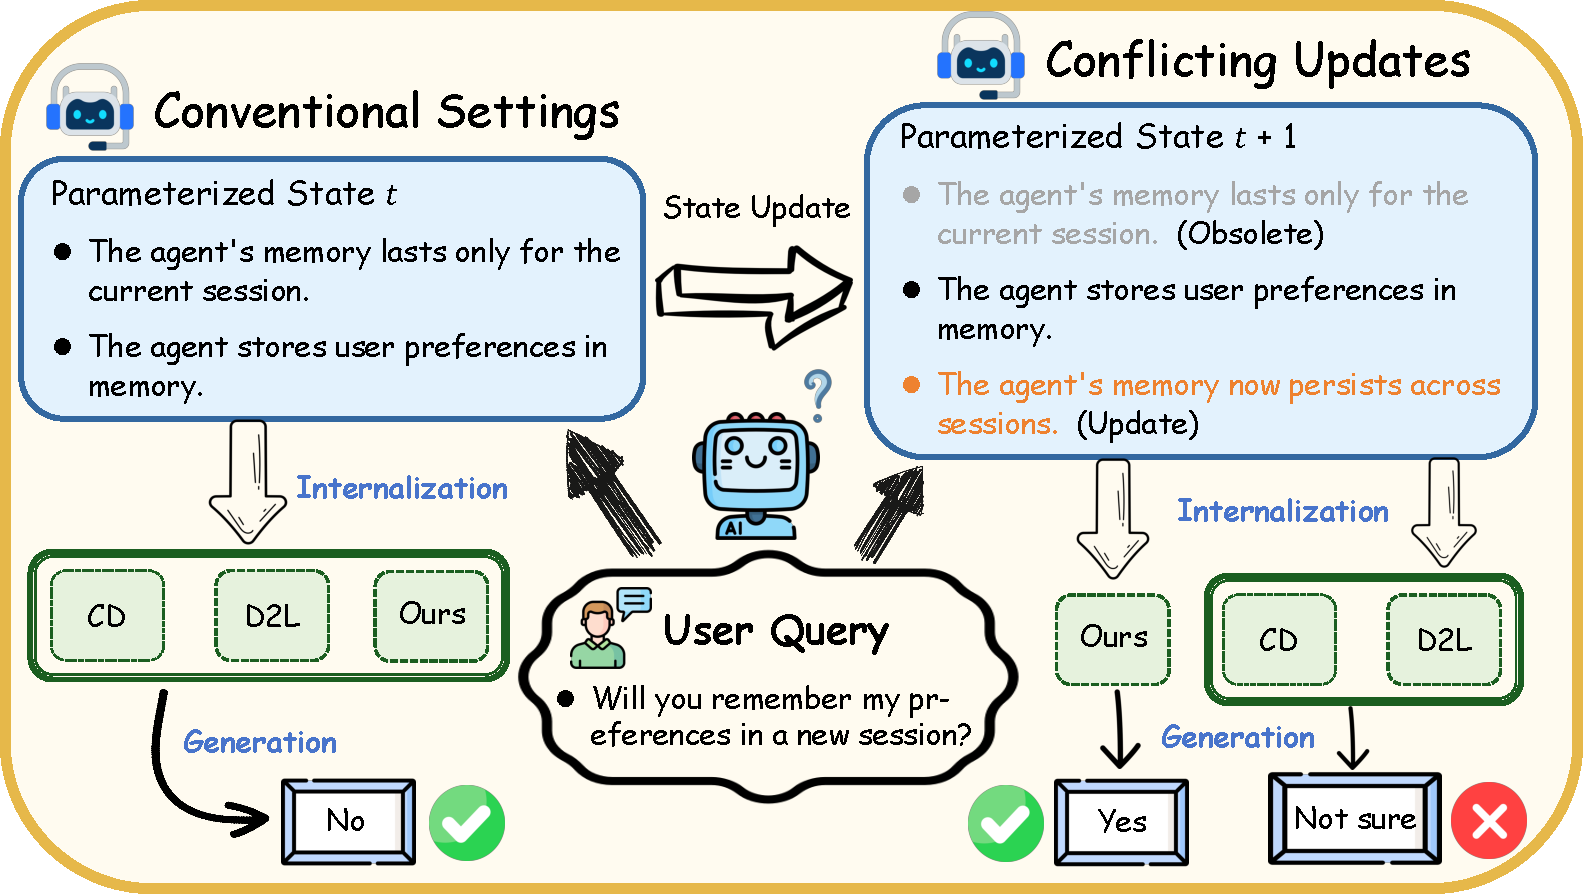
\includegraphics[
        width=\textwidth,
        % trim=14 83 14 84, % left, bottom, right, top
        clip
    ]{fig/intro/intro_quartz_crop.pdf}
    \caption{\textbf{Illustration of context parameterization under continual updates.}
    While existing methods perform well in conventional settings, they may conflate obsolete information with subsequent updates, whereas \method{} follows the currently valid information.
    }
    \label{fig:intro_motivation}
\end{figure*}

% P1
Large Language Models (LLMs) demonstrated remarkable general-purpose capabilities in question answering, reasoning, and text generation, advancing natural language processing~\citep{brown2020language,wei2022chain,guo2025deepseek}. 
Many practical tasks are context-intensive, requiring models to efficiently locate and reuse information from long contexts across successive queries~\citep{bai2024longbench,bai2025longbench,li2025scbench}.
Existing retrieval-augmented generation (RAG)~\citep{lewis2020retrieval,guu2020retrieval} and long-context methods~\citep{ding2023longnet} incur substantial inference overhead from repeated context processing~\citep{gao2023retrieval}, whereas context parameterization decouples this process from subsequent queries, enabling efficient reuse~\citep{snell2022learning,charakorn2026doc}.
Prior research followed two lines: \ding{172} one updated parametric knowledge through localized parameter modifications without retraining the model, as in knowledge editing~\citep{mitchell2022fast,meng2022locating,meng2023massediting}; \ding{173} the other internalized contextual information into reusable parameter representations, as in context distillation, Doc-to-LoRA, and SHINE, which compiled contexts into lightweight representations for subsequent queries~\citep{snell2022learning,charakorn2026doc,liu2026shine}.

% P2
Although these methods enabled effective, efficient context reuse, none addressed parameterization under evolving information validity~\citep{liu2025model,tian2026anyedit}.
In long-running agents and interactive systems, information continuously accumulates into persistent memory, making full context reconstruction impractical~\citep{park2023generative,packer2023memgpt,zhong2024memorybank}, motivating parameterized states that incorporate new information while preserving prior~\citep{jang2022temporalwiki}.
However, under continual updates, some information remains valid while other information is supplemented, replaced, or invalidated~\citep{wallat2026facts}, and jointly retaining information with different validity states can cause reliance on invalid information or inconsistent responses~\citep{marjanovic2024dynamicqa,wallat2026facts}.
Incorporating continual updates into a parameterized state while adhering to valid information thus remains an open challenge, as illustrated in Figure~\ref{fig:intro_motivation}: after an update, the parameterized state must incorporate updates while preserving what remains unaffected.

% P3
To study this continual-update setting, we formalized \textbf{Memory Updating with Sequential Evolution (\task{})} and designed a data construction pipeline preserving the original question and context structures, updating only the target and coupled information, and appending the updated context to the original.
This construction produces a context history with explicit update order and validity changes that supports the updated answer while no longer supporting the previous one.
Using this pipeline, we constructed \benchmark{} from five datasets, covering QA and reasoning.
Unlike prior work on conflicts between external context and model priors~\citep{xie2024adaptive,xu2024knowledge,kortukov2024studying}, \benchmark{} studies continual updates where valid and invalid information coexist within a parameterized state.
Experiments showed that parameterizing the full context into a unified representation substantially degraded performance, indicating severe interference among information with different validity states.

% P4
Building on \benchmark{}, we examined whether interference reflected information loss or merely suppressed activation by computing token-level ROUGE-L recall under teacher forcing for top-1 and top-5 candidate tokens at each step.
Top-5 recall reached \textbf{71.79}\%, far exceeding top-1's \textbf{45.90}\%, indicating valid information was largely retained in the output distribution but frequently outranked by invalid candidates. 
Thus, the observed interference was primarily a ranking rather than an information-loss problem. 
This finding motivates \method{}'s design: since the signal is present but underweighted, we first amplify the global representation; however, suppression varies across queries, so uniform amplification cannot precisely target which candidate to reweight and may override valid information, motivating query-activated memory evidence for precise, per-query correction. 
We retain the global representation rather than relying on local evidence alone because query-activated evidence can fail when a query's phrasing diverges from the original update context, lacking the cross-passage consistency encoded by the global representation. 
\method{} thus adaptively integrates both at decoding time---the global representation as a stable prior and memory evidence as a precise correction.

% P5
Experiments spanned multiple model families, including Qwen3 and Gemma2~\citep{yang2025qwen3,team2024gemma}, on five public state-update datasets, comparing \method{} with knowledge editing~\citep{jiang2025anyedit}, context distillation~\citep{askell2021general,snell2022learning}, Doc-to-LoRA~\citep{charakorn2026doc}, and other representative baselines.
Averaged across the five datasets, \method{} improved ROUGE-L Recall from \textbf{44.46} (D2L) to \textbf{57.76} (\textbf{13.30}$\uparrow$), and LLM-as-a-Judge from \textbf{34.49} to \textbf{53.41} (\textbf{18.92}$\uparrow$), while consistently outperforming all baselines across models and task settings.
These results demonstrated that \method{} effectively mitigated parametric interference among information with different validity states while improving adherence to currently valid information.
